
\chapter{User Manual}

\startcontents[chapters]
\printcontents[chapters]{}{1}{}

\section{Introduction}

\subsection{Purpose of System}

The purpose of the system is to provide an easy way to store data about hardware devices that are allocated to staff in the company. The system allows staff to view their own data, as well as certain staff being able to add, edit and remove data.

\textbf{The system achieves it's purpose with the following features:}

\underline{Different Access Levels}


\begin{itemize}
\item{The system has three different access levels which restrict access to certain parts of the system:}
	\begin{itemize}
	\item{Admin access level - The staff member will be able to access all parts of the system including adding,editing and removing data, creating graphs and viewing all staff members in the company.}
	\item{Manager access level - The staff member will have read only access to the system but will be able to view all staff records in their own department as well as send bug reports and data errors.}
	\item{Staff access level - The staff member will have read only access and only be able to view their own data in the system. They can send bug reports and data errors just as managers can.}
	\end{itemize}
\item{The system has an effective login system that requires all staff to use their login credentials in order to access the system. When creating user accounts IT staff can specify which access level they are granted}
\end{itemize}

\newpage
\underline{Ability store and search data}
\begin{itemize}
\item{As stated above, Admins can add, edit and remove data using a graphical interface}
\item{Staff member's can also search for data}
	\begin{itemize}
	\item Manager and Staff search functionality - Performed by entering a characters into a search box which will automatically filter data in the table to match search.
	\item{Admin search functionality - Performed by selecting a department and then searching for the staff member's first name. Users can then choose to view more information about this colleague. Admins can also perform searches using the search box on the tables (the same as Managers and Staff)}
	\end{itemize}
\end{itemize}

\underline{Graphical Analysis of Data}
\begin{itemize}
\item{Admins can create a bar chart representation of hardware sorted by department. By using a simple graphical button on the toolbar a bar chart will be created which will show how many hardware devices each department owns}
\end{itemize}

\underline{Email Functionality}
\begin{itemize}
\item{The system may be used by a variety of staff if they wish to check their own information. Because of this it is important for IT Staff to get feedback from other staff members about their experience with the system. Email functionality is used so staff can send bug reports and error reports to IT Staff members. It is important to make sure information is correct to ensure the company are abiding by the Data Protection Act}
\item{The system also has an automatic email that will be sent to IT Staff if a hardware device has 90 days left on the warranty}
\end{itemize}

\subsection{Intended Audience}

The intended audience for my system was staff at Volac International. More specifically my primary audience is IT Staff at Volac International, this is because they will be the main users of the system since the main purpose is to store and edit data. My secondary audience is other staff members who may use the system to view their own data, or department data in the case of managers.

\section{Installation}

\subsection{Prerequisite Installation}

%include as many subsubsections as necessary for each piece of required software
\subsubsection{Software}

My system has been compiled to a windows executable, therefore no software is needed prior to running the application.

\subsubsection{Hardware}

The system originally was designed to be stored onto a server with the following specs:

\begin{itemize}
\item HP DL360
\item Windows 2003 (can run any operating system required)
\item 4TB Hard Drive
\item 16GB RAM
\item Quad Core Processor - 2.5 GHZ
\end{itemize}

However after implementation the system is not currently able to allow multiple people to access the database at one time. A server may still be used to storage and should be required for future updates to my system which will eventually allow all staff to connect to the same database.

The server is stored in a server room with high ventilation and fans operated 24/7. This is a huge benefit because the system can be running at all times so people can access the database. Preferably the overall model will be client-server and each user will have their own login for security. All users should connect using clients on local computers and will not directly access the server.

Users will connect to the system using their own computers at the workplace. These computers all have Windows 7 installed and run at the resolution of 1920x1080. The monitor sizes range from different locations, but the smallest would be 21" LCD monitors and the largest would be 27". These sizes will not be a problem since the application will be designed to fit on these monitors. All computers have a mouse, which is required for clicking the interface buttons, and a keyboard which is required for entering information. This system will not be developed for touch screen devices. The data for the program (if stored on the server) will be held on a hard drive inside the server that can be accessed by everyone who is connected to it. The company will not need any additional hardware to run the proposed system.

\subsubsection{Operating System}

The system has been developed using both Macintosh OS and Windows (64 bit and 32 bit). However since adding some functions the system does not seem to be functioning correctly on Mac while deleting and searching for staff (in the Admin Interface). The program has also been compiled onto a Windows Executable (.exe) which means that a machine running Windows is required, this works for both 32 bit and 64 bit machines.

\subsection{System Installation}\label{systeminstall}

In order to install the system onto your computer, please follow the steps below:

\textbf{1) Navigate to the directory where you saved the installer, I will be using a folder called "/Tutorial" but it will be different on your computer.}

\begin{figure}[H]
    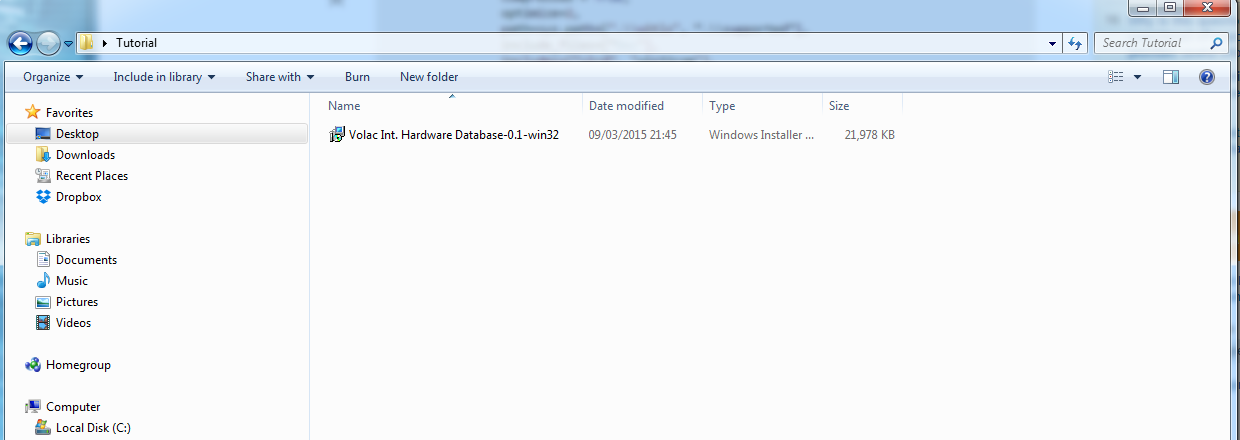
\includegraphics[width=\textwidth]{./Manual/Images/Tut1.png}
\end{figure}

\textbf{2) Double click the installer (left mouse button) and the setup will begin.}

\newpage

\textbf{3) The following window will appear, from here you may choose the location for the system to be installed to. By default it should install to "Program Files" for 32 bit computers or "Program File (x86)" for 64 bit computers.}

\begin{figure}[H]
    \includegraphics[width=\textwidth]{./Manual/Images/Tut2.png}
\end{figure}

\newpage

\textbf{4) Press the "Next" button to start the installation.}

\begin{figure}[H]
    \includegraphics[width=\textwidth]{./Manual/Images/Tut3.png}
\end{figure}

\newpage

\textbf{5) If the following warning message appears, press the "Yes" button to give permission for the installation to continue.}

\begin{figure}[H]
    \includegraphics[width=\textwidth]{./Manual/Images/Tut4.png}
\end{figure}

\newpage

\textbf{6) The installation should now begin. If the installer is no longer open, please see "step 2".}

\begin{figure}[H]
    \includegraphics[width=\textwidth]{./Manual/Images/Tut5.png}
\end{figure}

\newpage

\textbf{7) Press the "Finish" button after the installation has finished.}

\begin{figure}[H]
    \includegraphics[width=\textwidth]{./Manual/Images/Tut6.png}
\end{figure}

\newpage

\textbf{8) Navigate to the location the system was installed to and a folder called "Volac Int. Hardware Database" should be present.}

\begin{figure}[H]
    \includegraphics[width=\textwidth]{./Manual/Images/Tut7.png}
\end{figure}

\textbf{9) The program is now installed. The next section \ref{runprogram} will explain how to run your new system.}

\subsection{Running the System}\label{runprogram}

This section will be looking at how to run the system. If you have not yet installed the system onto your machine, please see the above section \ref{systeminstall}.

\newpage

\textbf{1) Locate the Windows Executable in the location where the system was installed.}

\begin{figure}[H]
    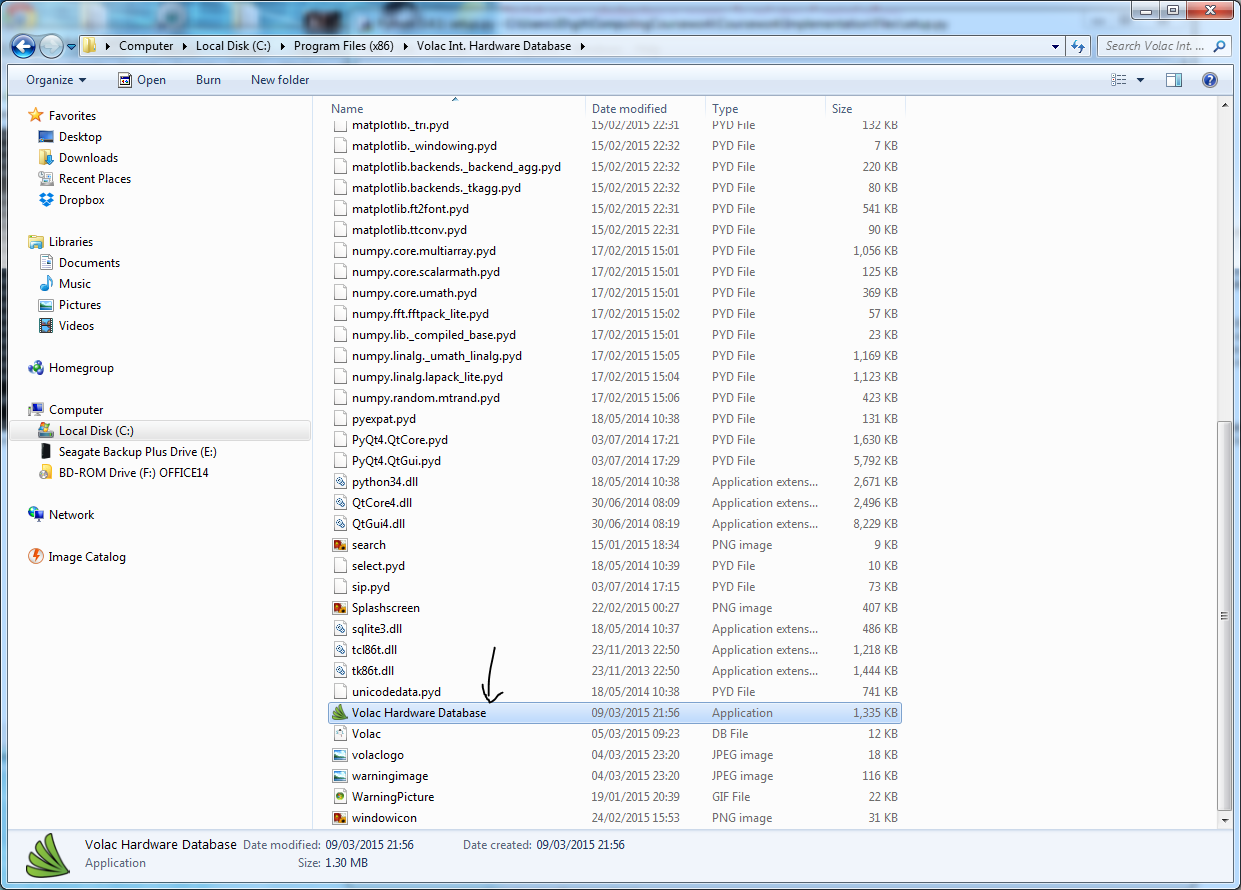
\includegraphics[width=\textwidth]{./Manual/Images/run1.png}
\end{figure}

\newpage

\textbf{Optional Step: 1.1) It is recommended that you create a shortcut so that it can be ran easier in the future. To do this "Right Click" the Executable and "Left Click" the "Create Shortcut" option.}

\begin{figure}[H]
    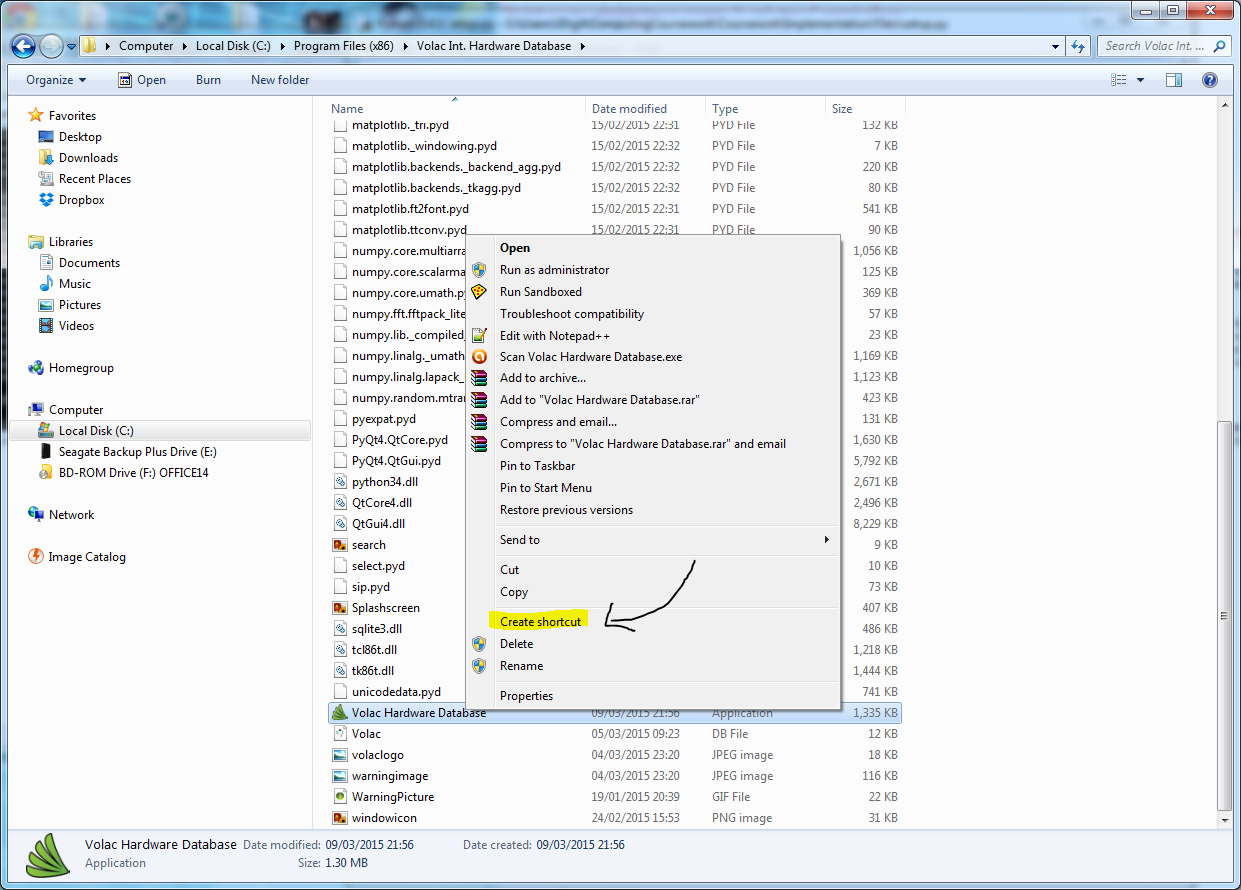
\includegraphics[width=\textwidth]{./Manual/Images/run2.png}
\end{figure}

\textbf{Optional Step: 1.2) The following warning message should appear. After clicking "Yes" a shortcut should be placed onto the Desktop.}

\begin{figure}[H]
    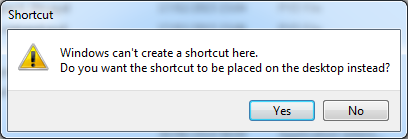
\includegraphics[width=\textwidth]{./Manual/Images/run3.png}
\end{figure}
\newpage

\textbf{Optional Step: 1.3) If the shortcut was created successfully an Executable should now be on your Desktop.}

\begin{figure}[H]
    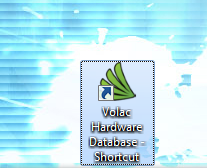
\includegraphics[width=\textwidth]{./Manual/Images/run4.png}
\end{figure}
\newpage

\textbf{2) Double click the Executable, either the original, or the shortcut if the above steps were followed.  If done correctly, the following screen should appear.}

\begin{figure}[H]
    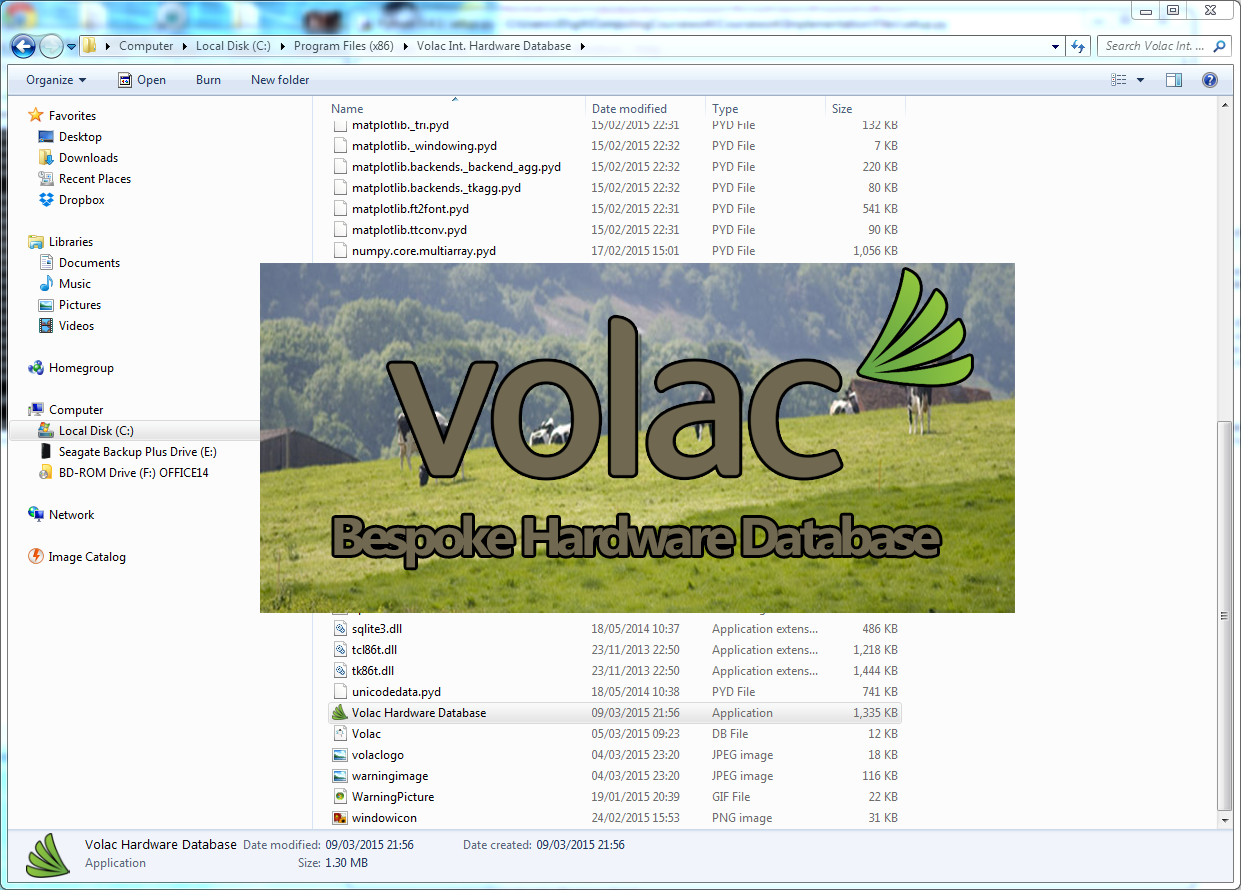
\includegraphics[width=\textwidth]{./Manual/Images/run5.png}
\end{figure}

\newpage

\textbf{3) After the program has loaded, the login screen should appear. The default Admin login will be: \newline
Username: "Admin" \newline
Password: "password"}

\begin{figure}[H]
    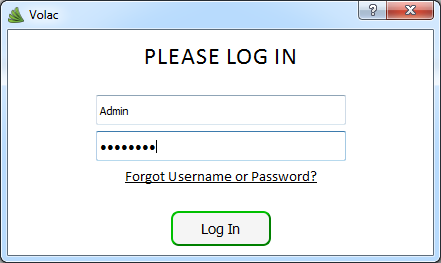
\includegraphics[width=\textwidth]{./Manual/Images/run6.png}
\end{figure}

\textbf{4) The program is now running and you should be able to gain access to the Admin Interface below.}

\begin{figure}[H]
    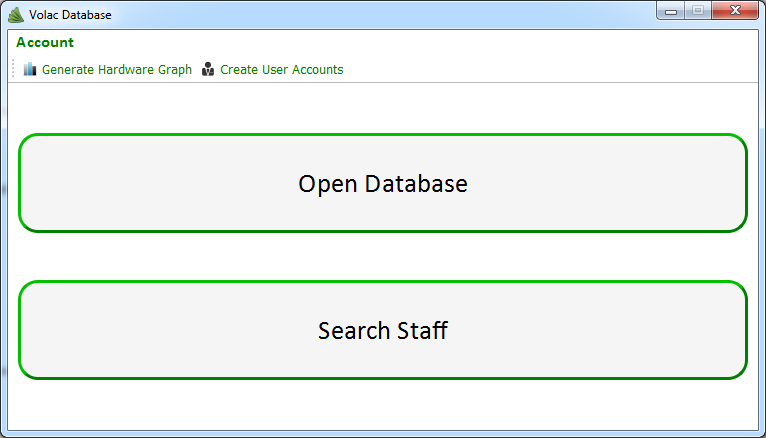
\includegraphics[width=\textwidth]{./Manual/Images/run7.png}
\end{figure}

\section{Tutorial}

\subsection{Introduction}

In this section I will be explaining how to use each part of the system. All tutorials have a step-by-step guide with annoted images to assist you in the best possible way.

\subsection{Assumptions}

I will assume that there is no prior knowledge of using computers since staff members at Volac International will have mixed levels of understanding to computer systems. To follow the tutorial the program must be already up and running, if it is not please follow the guide for "Running the System" \ref{runprogram}

\subsection{Tutorial Questions}

The following tutorials are split into a question and answer format. They are also split up to help specific access levels.

\textbf{General Questions}

\begin{center}
    \begin{longtable}{|p{5cm}|p{2cm}|p{2cm}|}
        \hline
        \textbf{Question} & \textbf{Question Number} & \textbf{Page Number} \\ \hline
How do I login to the system? & \ref{howlogin} & \pageref{howlogin} \\ \hline
How do I change my password? & \ref{changepass} & \pageref{changepass}\\ \hline
How do I close the system? & \ref{closesys} & \pageref{closesys}\\ \hline
	\end{longtable}
\end{center}

\textbf{Admin Questions}

\begin{center}
    \begin{longtable}{|p{5cm}|p{2cm}|p{2cm}|}
        \hline
        \textbf{Question} & \textbf{Question Number} & \textbf{Page Number} \\ \hline
How do I open the database? & \ref{opendb} & \pageref{opendb}\\ \hline
How do I view the different tables in the database? & \ref{viewdb} & \pageref{viewdb}\\ \hline
How do I add data to the database? & \ref{adddata} & \pageref{adddata}\\ \hline
How do I edit data in the database? & \ref{editdata} & \pageref{editdata}\\ \hline
How do I delete data from the database?  & \ref{deletedata} & \pageref{deletedata}\\ \hline
How do I quick search for data in the database? & \ref{quicksearch} & \pageref{quicksearch}\\ \hline
How do I search for staff by department? & \ref{departsearch} & \pageref{departsearch}\\ \hline
How do I generate a graph? & \ref{graph} & \pageref{graph}\\ \hline
How do I add new accounts to the system? & \ref{accountcreate} & \pageref{accountcreate}\\ \hline
What are primary and foreign keys and how do I use them? & \ref{keys} & \pageref{keys}\\ \hline

	\end{longtable}
\end{center}

\textbf{Manager and Staff Questions}

\begin{center}
    \begin{longtable}{|p{5cm}|p{2cm}|p{2cm}|}
        \hline
        \textbf{Question} & \textbf{Question Number} & \textbf{Page Number} \\ \hline
I forgot my password, how do I recover it? & \ref{recoveraccount} & \pageref{recoveraccount}\\ \hline
How do I view staff in my department? & \ref{department} & \pageref{department}\\ \hline
How do I quick search for data when viewing Department Information? & \ref{departquicksearch} & \pageref{departquicksearch}\\ \hline
How do I view my own information?  & \ref{owninfo} & \pageref{owninfo}\\ \hline
How do I report a bug? & \ref{bugreport} & \pageref{bugreport}\\ \hline
How do I report incorrect information? & \ref{incorrectinfo} & \pageref{incorrectinfo}\\ \hline

	\end{longtable}
\end{center}

%include as many subsubsections as necessary for each question in your list
\paragraph{General Tutorial}

\subsubsection{How do I login to the system?}\label{howlogin}

To log in to the system you will first be required to have a user account. If you have data in the database then the IT Staff should have provided you with a login.

1) Open the system

2) Fill out your username and password

\begin{figure}[H]
    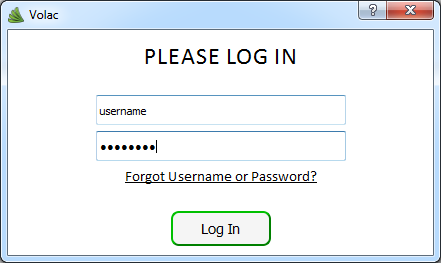
\includegraphics[width=\textwidth]{./Manual/Images/login1.png}
\end{figure}

3) Press Log In

\begin{figure}[H]
    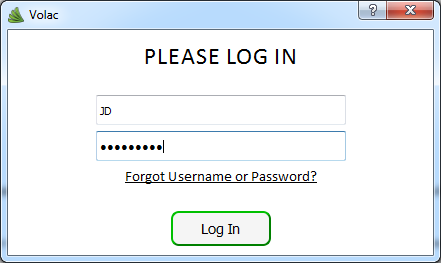
\includegraphics[width=\textwidth]{./Manual/Images/login2.png}
\end{figure}


If you have data but do not know your account. See section \ref{recoveraccount}

\subsubsection{How do I change my password?}\label{changepass}

1) Login to your interface

2) Locate and press the account menu on the menubar

\begin{figure}[H]
    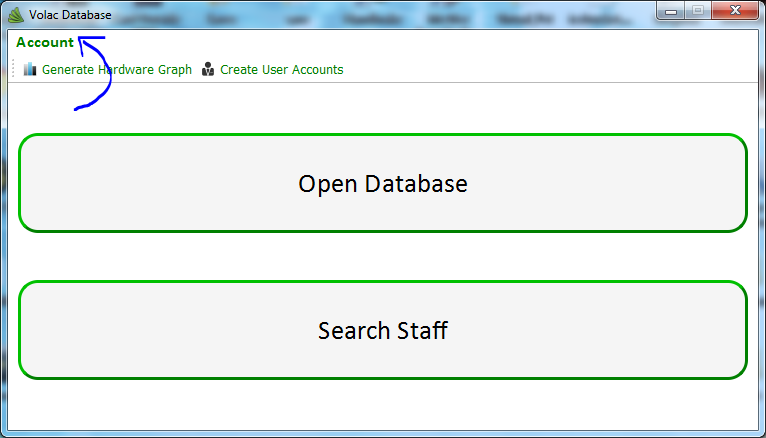
\includegraphics[width=\textwidth]{./Manual/Images/changepass.png}
\end{figure}

3) Click "Change Password"

\begin{figure}[H]
    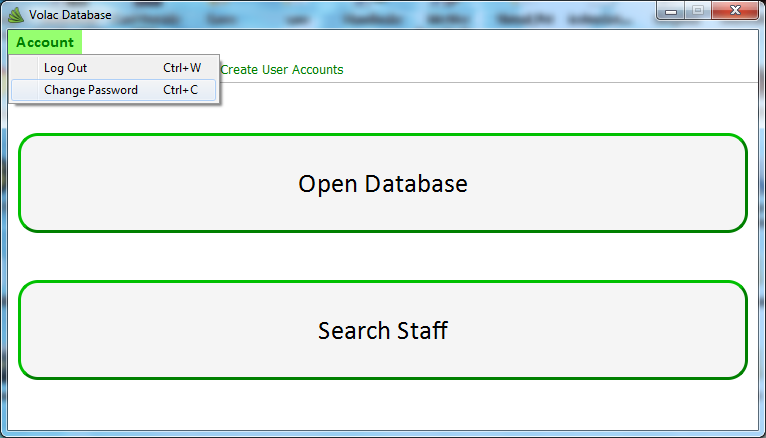
\includegraphics[width=\textwidth]{./Manual/Images/changepass2.png}
\end{figure}

4) Fill out the fields and click "Change", if done successfully, the confirmation message will appear under the buttons (shown below)

\begin{figure}[H]
    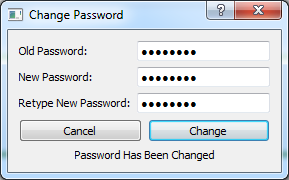
\includegraphics[width=\textwidth]{./Manual/Images/changepass3.png}
\end{figure}


\subsubsection{How do I close the system?}\label{closesys}

You may close the system at any time in three different ways:

\begin{itemize}
\item{Pressing the "X" button on the window}

\begin{figure}[H]
    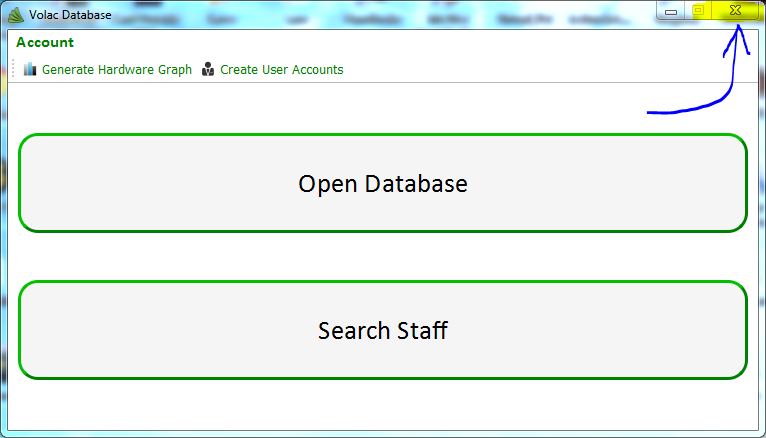
\includegraphics[width=\textwidth]{./Manual/Images/close2.png}
\end{figure}

\item{Going to the account menu and pressing "Log Out"}

\begin{figure}[H]
    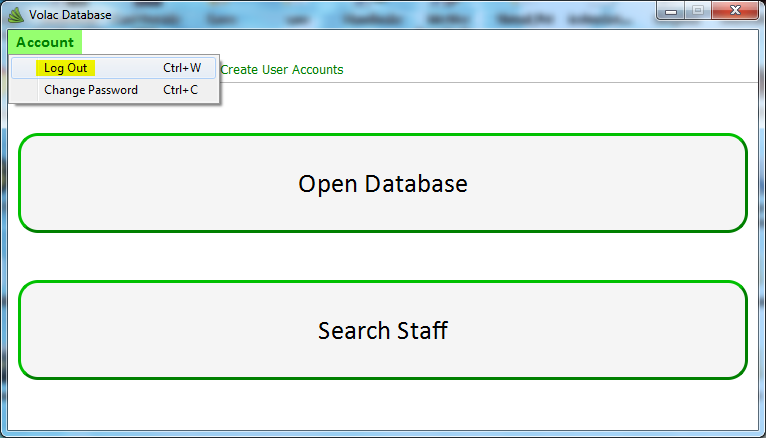
\includegraphics[width=\textwidth]{./Manual/Images/close1.png}
\end{figure}

\item{Using the keyboard shortcut "CTRL+W}

\begin{figure}[H]
    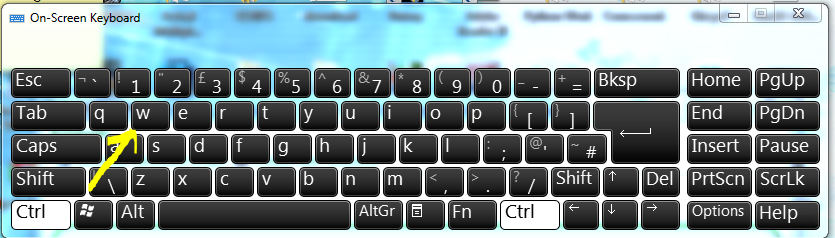
\includegraphics[width=\textwidth]{./Manual/Images/close3.png}
\end{figure}

\end{itemize}

Please bare in mind that the system does not have an autosave feature, make sure all data is saved before closing.

\paragraph{Admin Interface Tutorial}

\subsubsection{How do I open the database?}\label{opendb}

1) From the main menu click the "Open Database" button

\begin{figure}[H]
    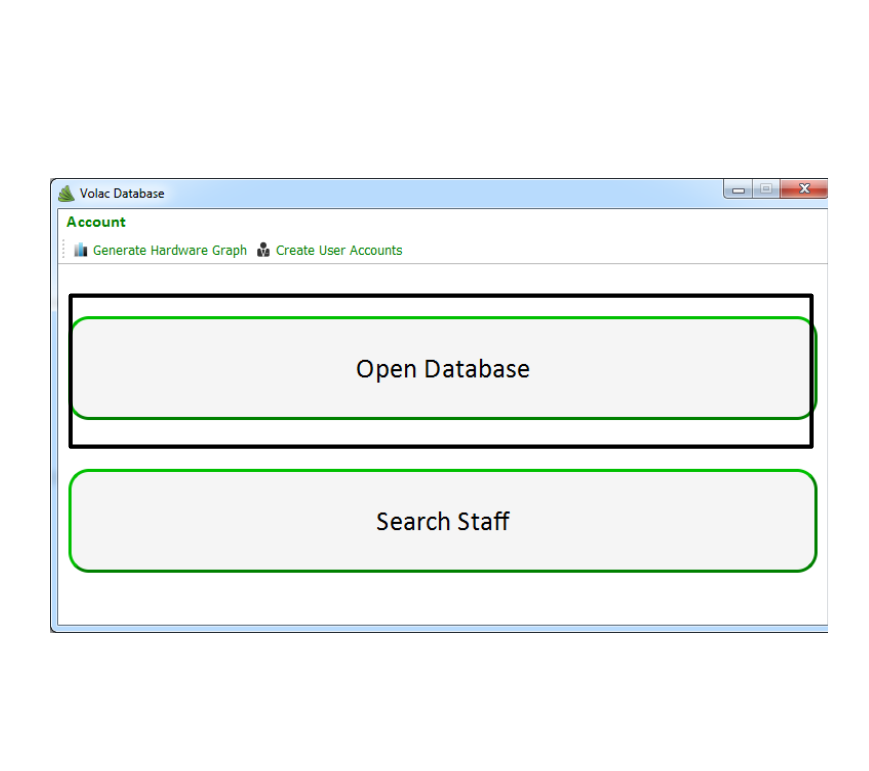
\includegraphics[width=\textwidth]{./Manual/Images/opendb1.png}
\end{figure}


2) Click the "Open Database"  button (next to the "Select Table" dropdown box)

\begin{figure}[H]
    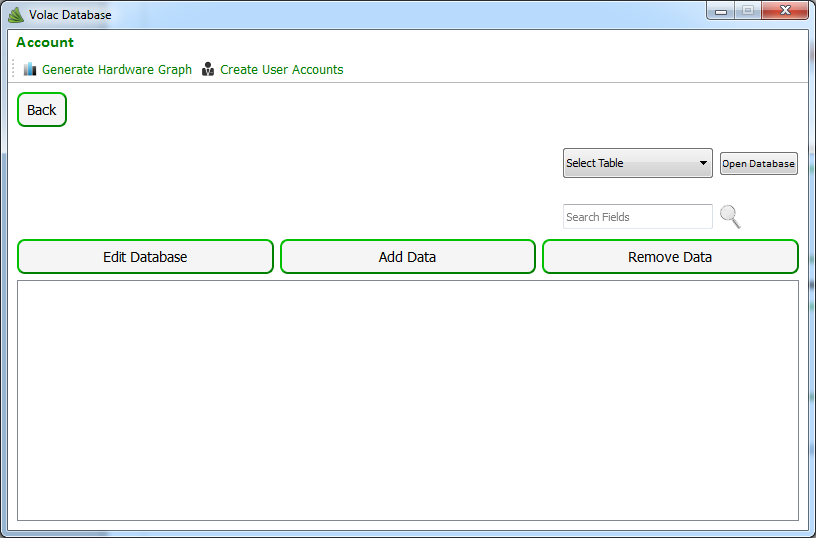
\includegraphics[width=\textwidth]{./Manual/Images/opendb2.png}
\end{figure}


3) Choose the correct database file, it will be named "Volac.db". 

\begin{figure}[H]
    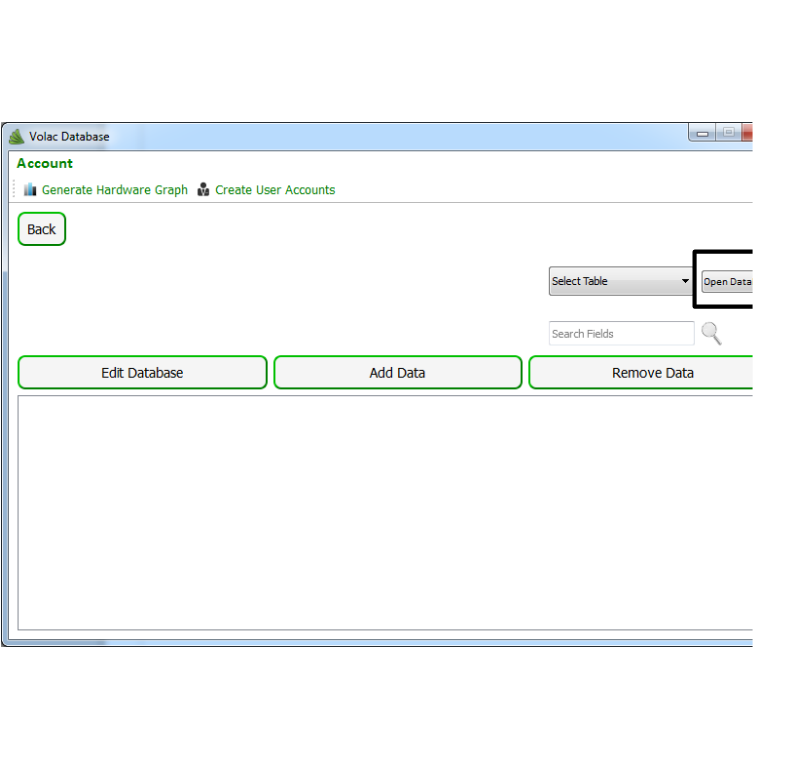
\includegraphics[width=\textwidth]{./Manual/Images/opendb3.png}
\end{figure}

4) The database is now open


\subsubsection{How do I view the different tables in the database?}\label{viewdb}

1) Open the database (follow the above tutorial \ref{opendb} if you need help doing this)

2) Press the dropdown box named "Select Table" 

\begin{figure}[H]
    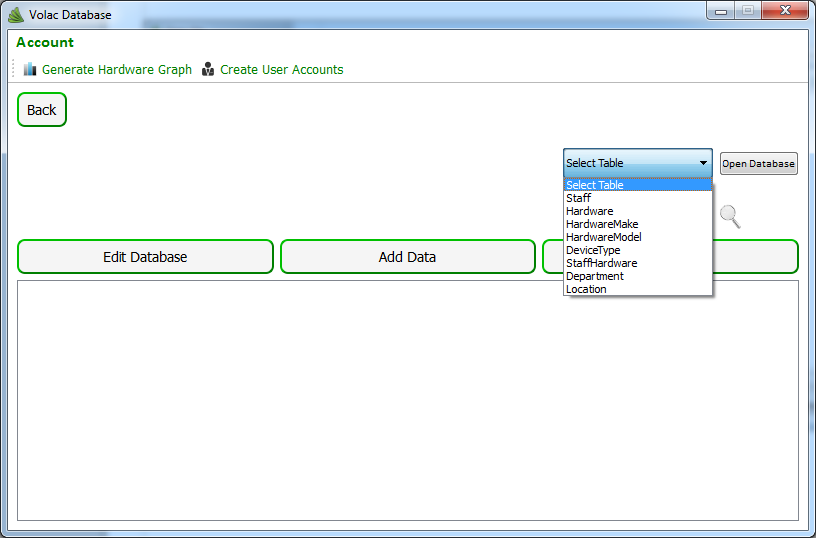
\includegraphics[width=\textwidth]{./Manual/Images/table1.png}
\end{figure}

3) Select the desired table to view it

\begin{figure}[H]
    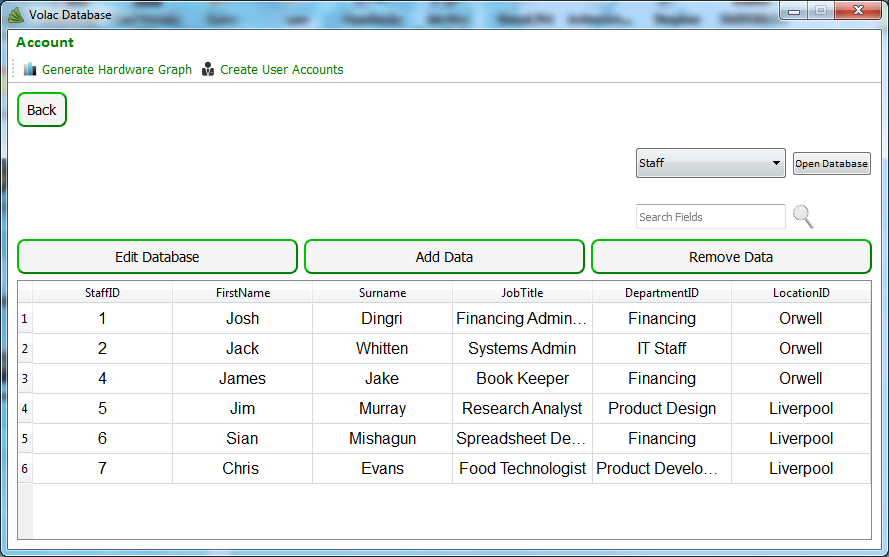
\includegraphics[width=\textwidth]{./Manual/Images/tabl2.png}
\end{figure}

\subsubsection{How do I add data to the database?}\label{adddata}

1) Open the database (\ref{opendb})

2) Select the table of your choice (\ref{viewdb})

3) Press the "Add Data" button

\begin{figure}[H]
    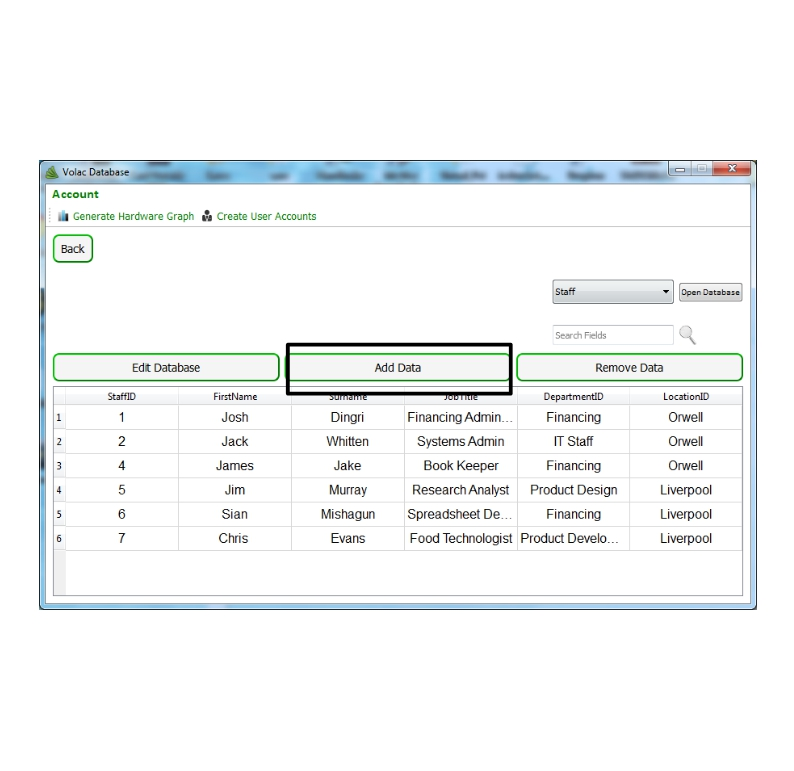
\includegraphics[width=\textwidth]{./Manual/Images/adddata.jpg}
\end{figure}

4) Fill out all the required fields, the fields will turn green if the entry is valid

\begin{figure}[H]
    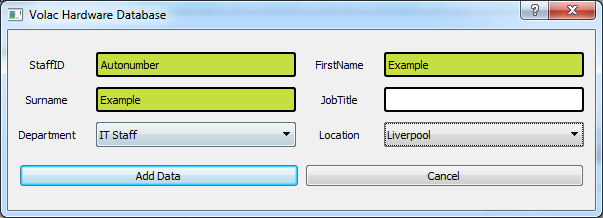
\includegraphics[width=\textwidth]{./Manual/Images/adddata2.png}
\end{figure}

5) Press "Add Data" to add the information to the database, the window should close and the table should automatically update

\begin{figure}[H]
    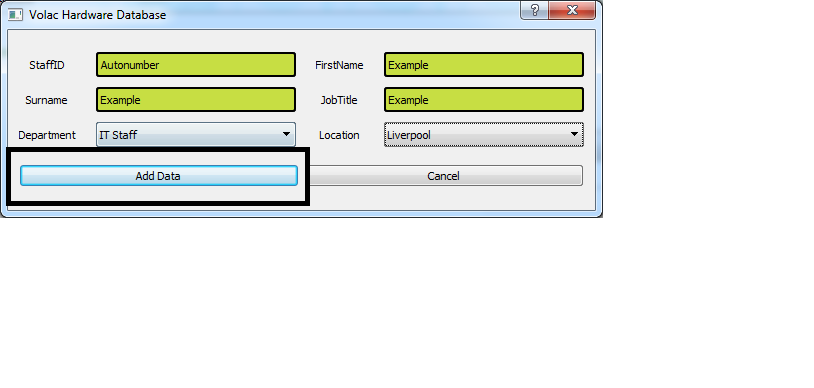
\includegraphics[width=\textwidth]{./Manual/Images/adddata3.png}
\end{figure}

\begin{figure}[H]
    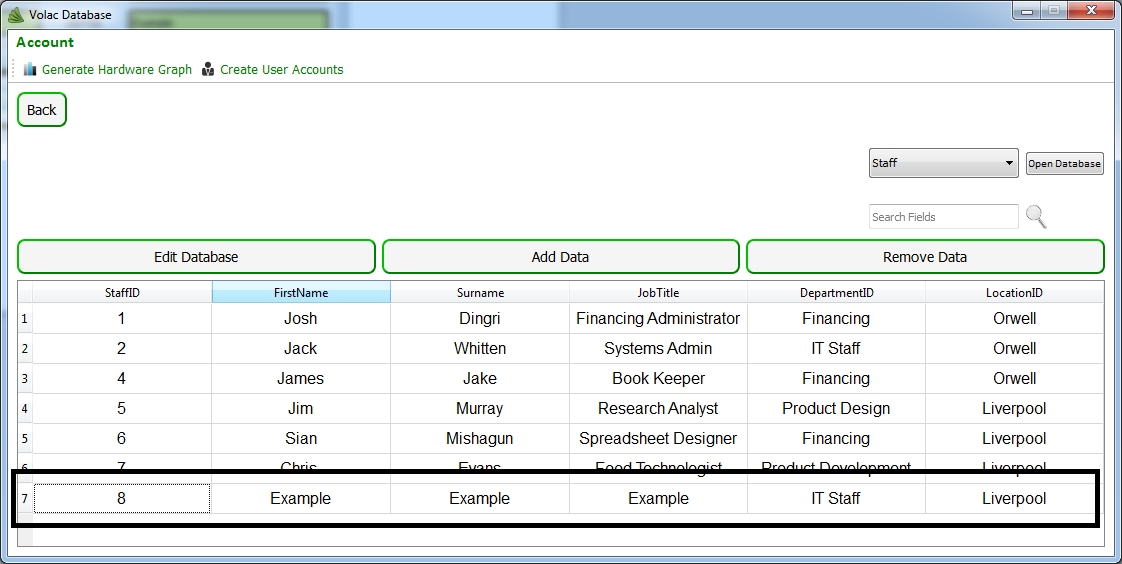
\includegraphics[width=\textwidth]{./Manual/Images/adddata4.png}
\end{figure}

\subsubsection{How do I edit data in the database?}\label{editdata}

1) Open the database (\ref{opendb})

2) Select the table of your choice (\ref{viewdb})

3) Press the "Edit Database" button 

\begin{figure}[H]
    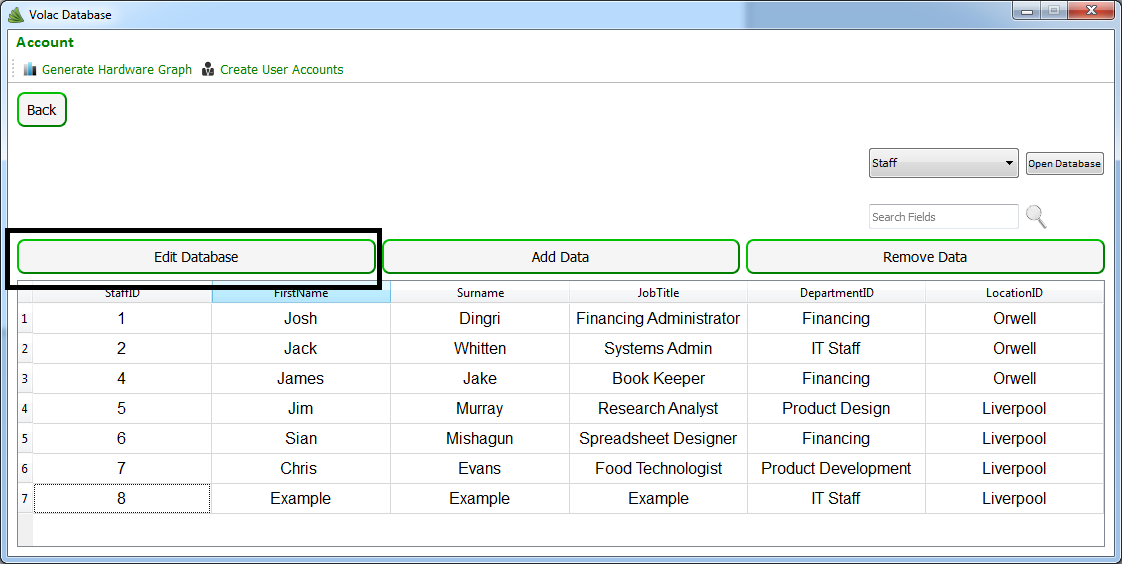
\includegraphics[width=\textwidth]{./Manual/Images/editdata.png}
\end{figure}

4) You may now change any fields of your choice, make sure the foreign keys (See \ref{keys}) (digits under certain 'ID Fields') are changed only to reference primary keys of other tables.

5) After a field has been changed press the "Enter" button on your keyboard to exit the field.

\begin{figure}[H]
    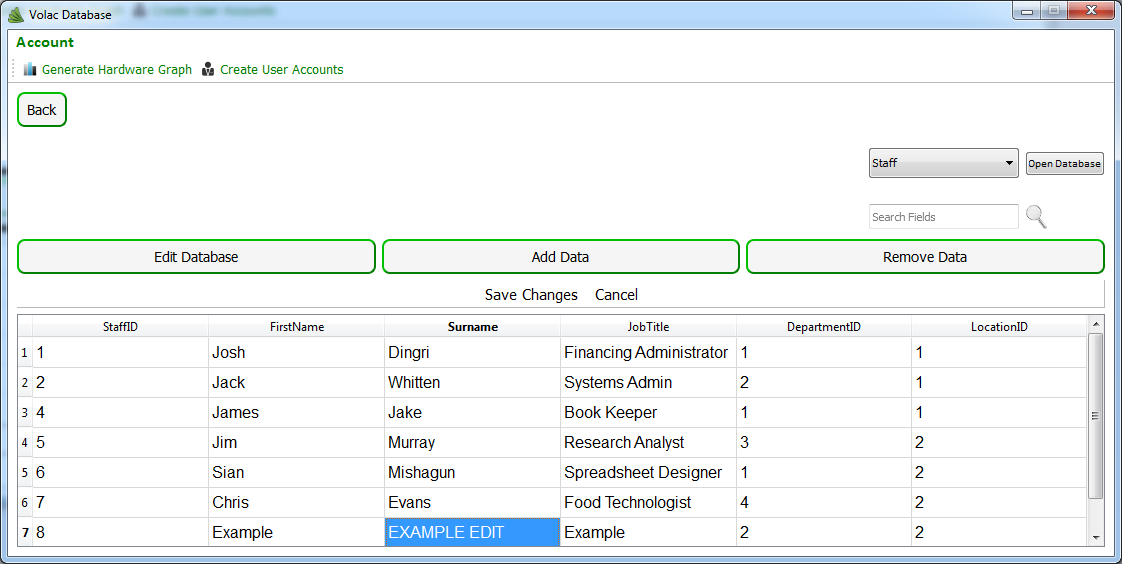
\includegraphics[width=\textwidth]{./Manual/Images/editdata2.png}
\end{figure}

6) After all desired fields have been changed you can either press the "Cancel" button to revert back to read only view without saving. Or the "Save Changes" button to save all changes and revert back to read only view.

\begin{figure}[H]
    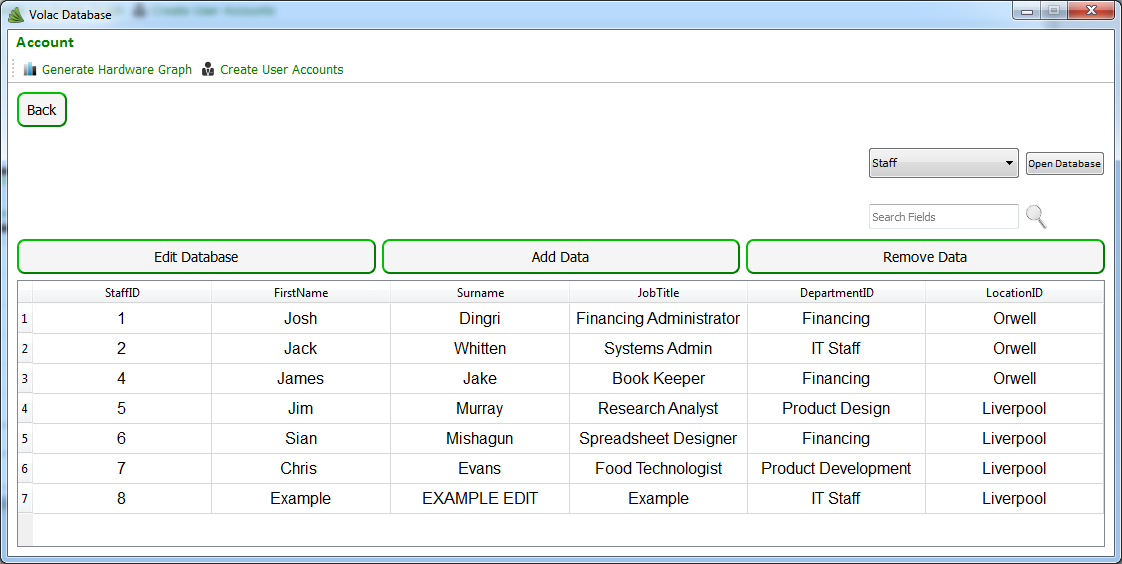
\includegraphics[width=\textwidth]{./Manual/Images/editdata3.png}
\end{figure}

\subsubsection{How do I delete data from the database?}\label{deletedata}

1) Open the database (\ref{opendb})

2) Select the table of your choice (\ref{viewdb})

3) Press the "Remove Data" button

\begin{figure}[H]
    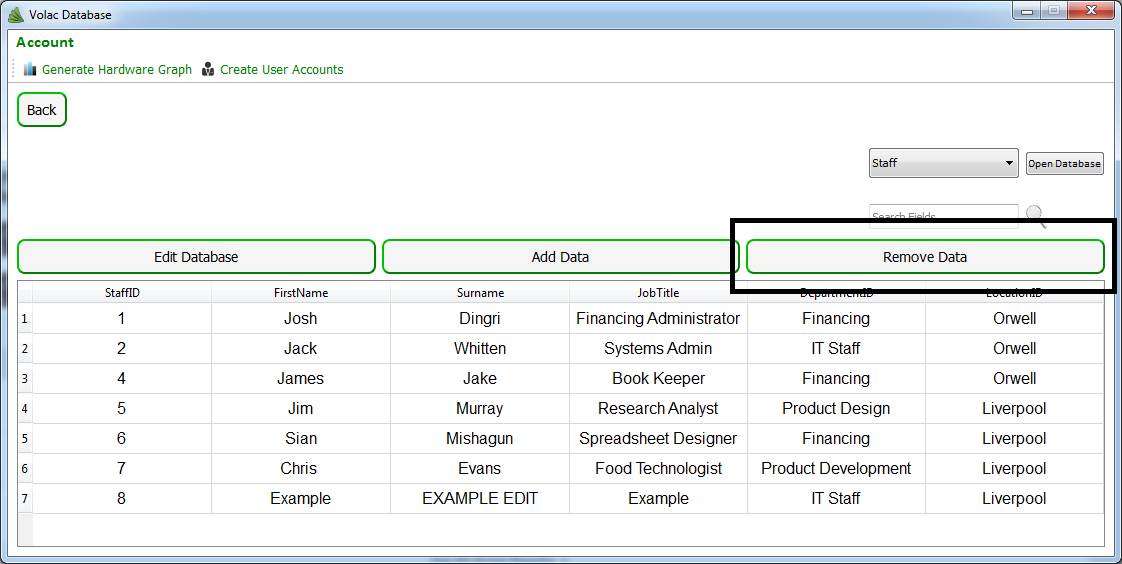
\includegraphics[width=\textwidth]{./Manual/Images/deletedata.png}
\end{figure}

4) To delete a record you may click the "Delete" button, this will delete the entire record of data

\begin{figure}[H]
    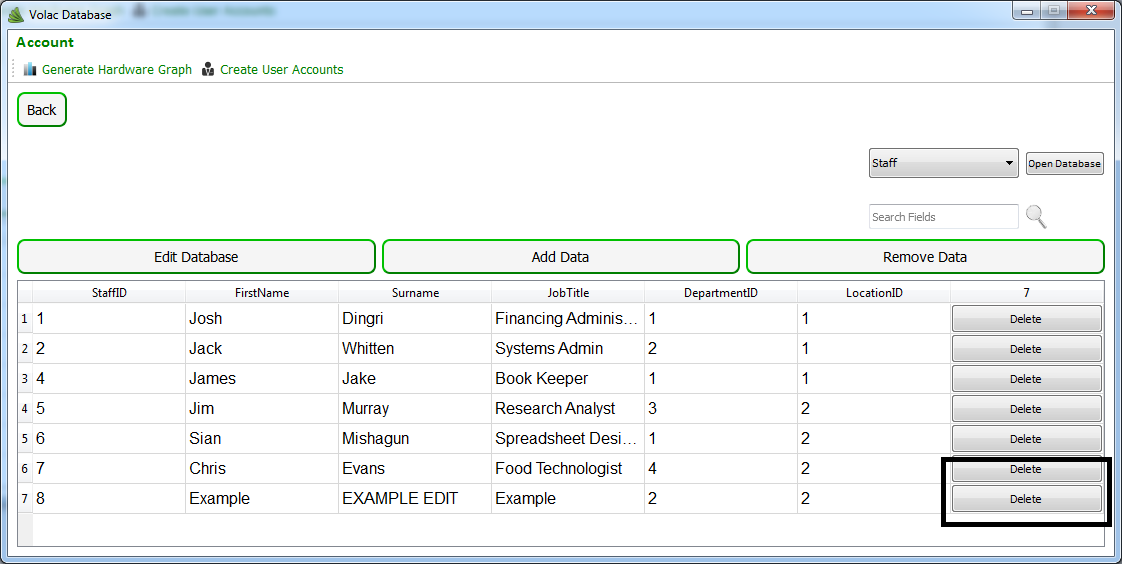
\includegraphics[width=\textwidth]{./Manual/Images/deletedata2.png}
\end{figure}

5) A warning message will appear, to confirm deletion. Click "Yes" to confirm deletion

\begin{figure}[H]
    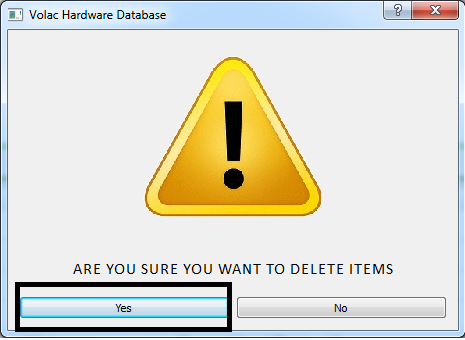
\includegraphics[width=\textwidth]{./Manual/Images/deletedata3.png}
\end{figure}

6) To revert back to read only view click the "Remove Data" button again

\begin{figure}[H]
    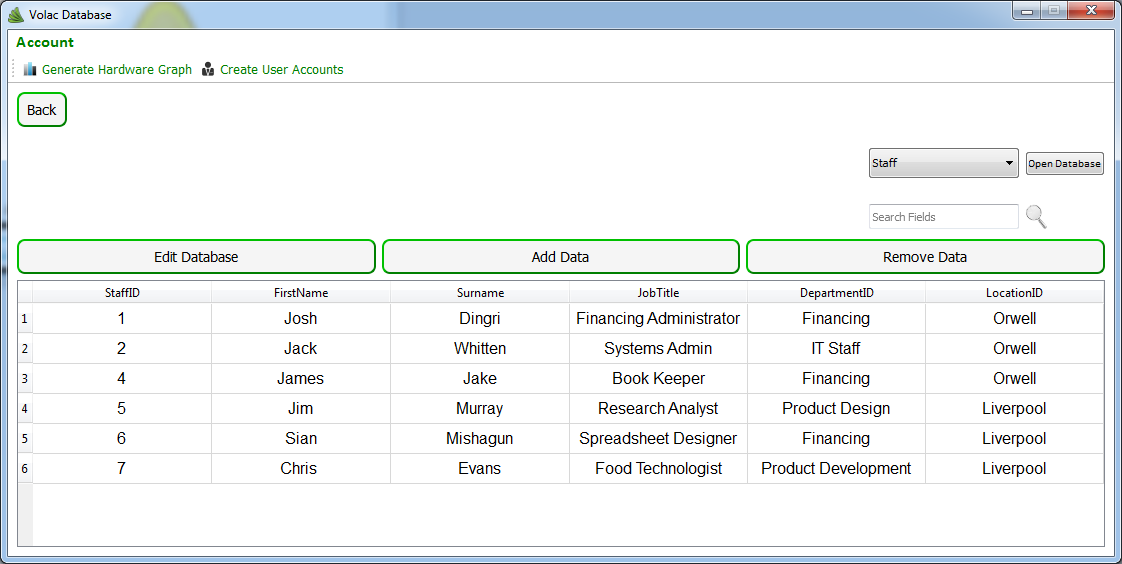
\includegraphics[width=\textwidth]{./Manual/Images/deletedata4.png}
\end{figure}


\subsubsection{How do I quick search for data in the database?}\label{quicksearch}

1) Open the database (\ref{opendb})

2) Select the table of your choice (\ref{viewdb})

3) To search for a field, enter text into the search box 

\begin{figure}[H]
    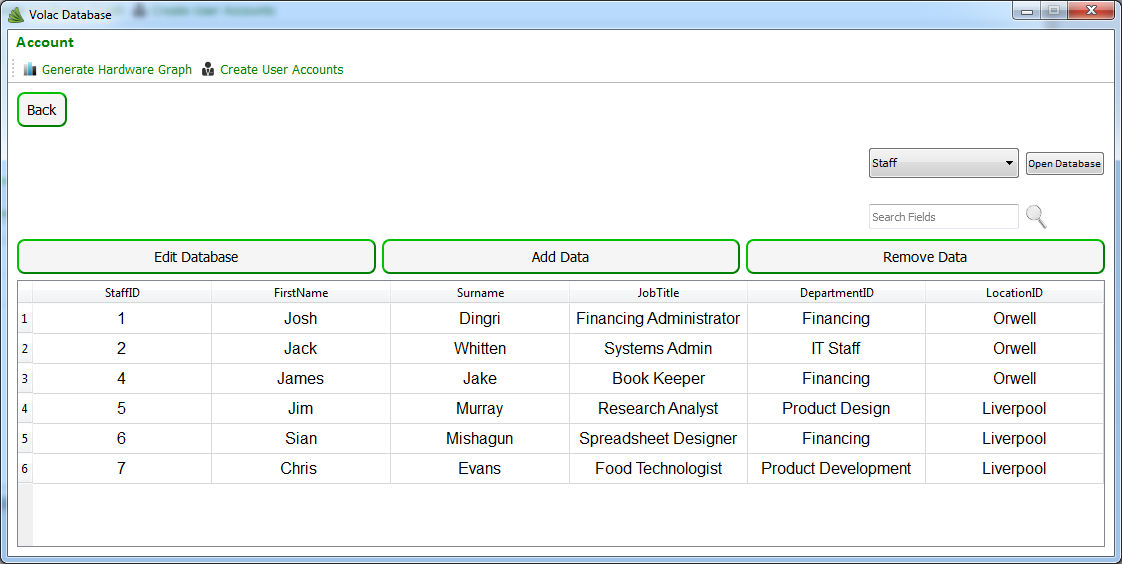
\includegraphics[width=\textwidth]{./Manual/Images/search1.png}
\end{figure}

4) The table will automatically filter to show the text input

\begin{figure}[H]
    
\includegraphics[width=\textwidth]{./Manual/Images/search.png}
\end{figure}

5) To show the whole table again, remove the text in the search box

\begin{figure}[H]
    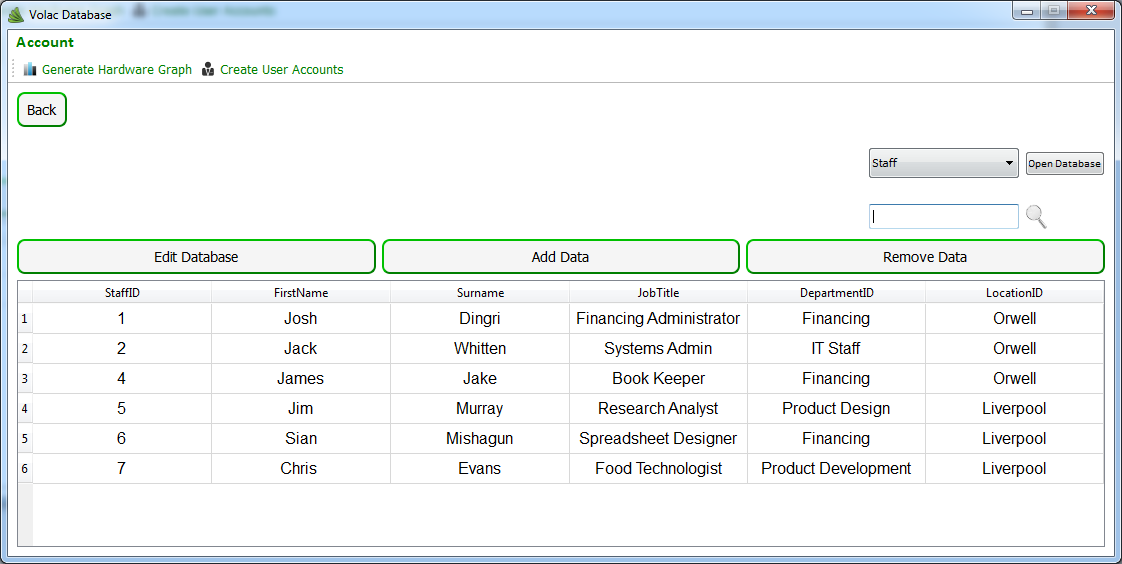
\includegraphics[width=\textwidth]{./Manual/Images/search2.png}
\end{figure}


\subsubsection{How do I search for staff by department?}\label{departsearch}

1) From the main menu press the "Search Staff" button

\begin{figure}[H]
    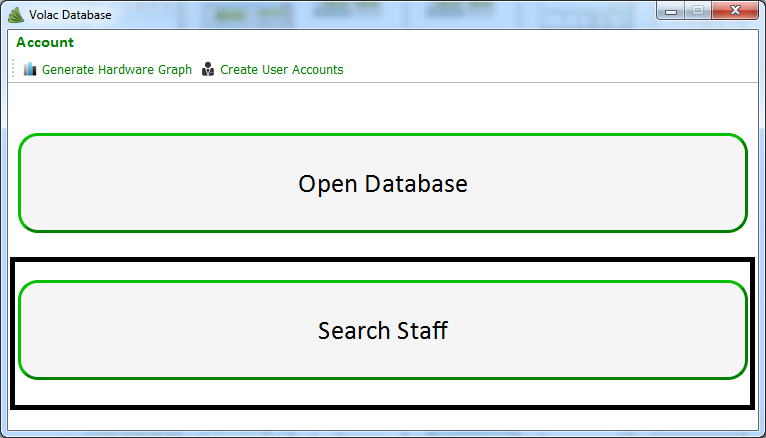
\includegraphics[width=\textwidth]{./Manual/Images/searchdep.png}
\end{figure}

2) Select the department using the drop down box, this will display all staff from the specified department

\begin{figure}[H]
    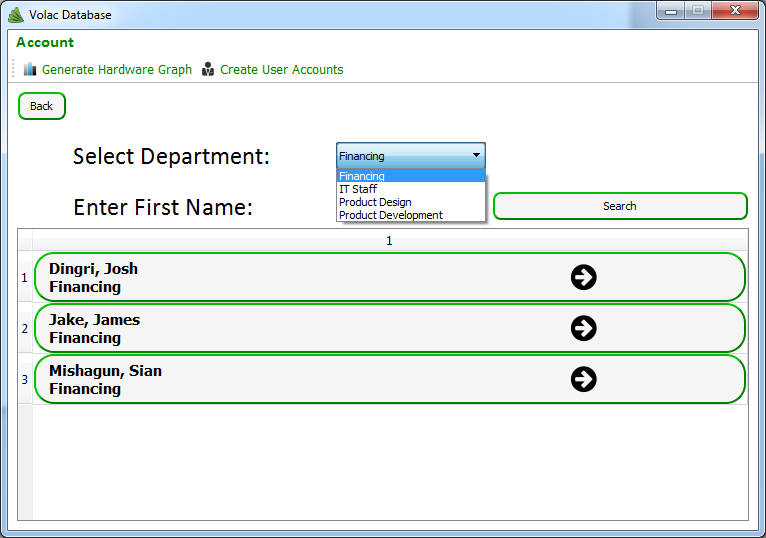
\includegraphics[width=\textwidth]{./Manual/Images/searchdep2.png}
\end{figure}

3) To search for staff member enter their first name in the search box

\begin{figure}[H]
    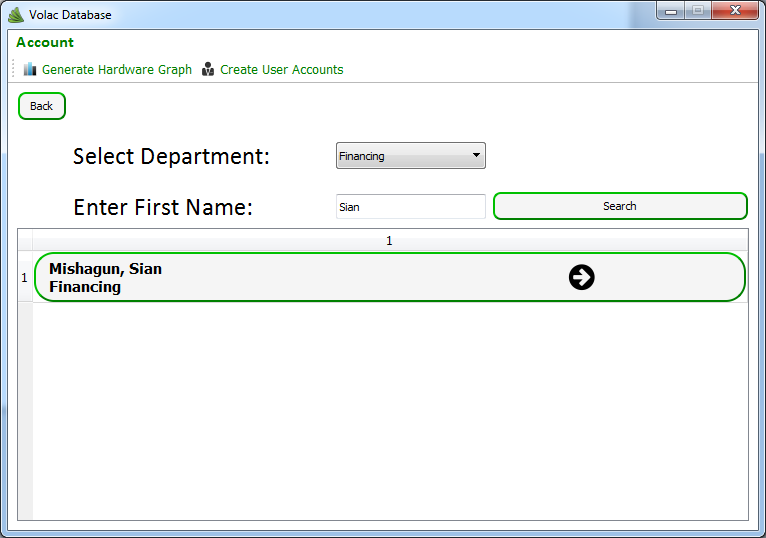
\includegraphics[width=\textwidth]{./Manual/Images/searchdep3.png}
\end{figure}

4) To get further information about the staff member click their button

\begin{figure}[H]
    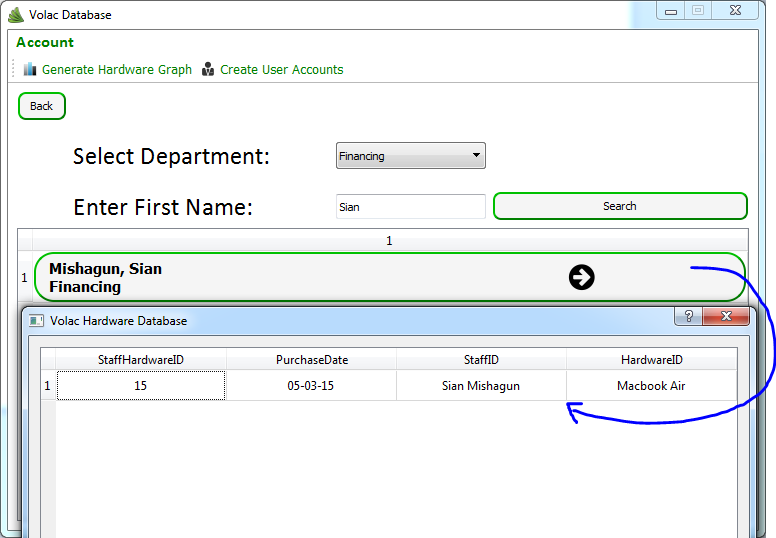
\includegraphics[width=\textwidth]{./Manual/Images/searchdep4.png}
\end{figure}

\subsubsection{How do I generate a graph?}\label{graph}

1) From anywhere in the Admin interface locate the toolbar

\begin{figure}[H]
    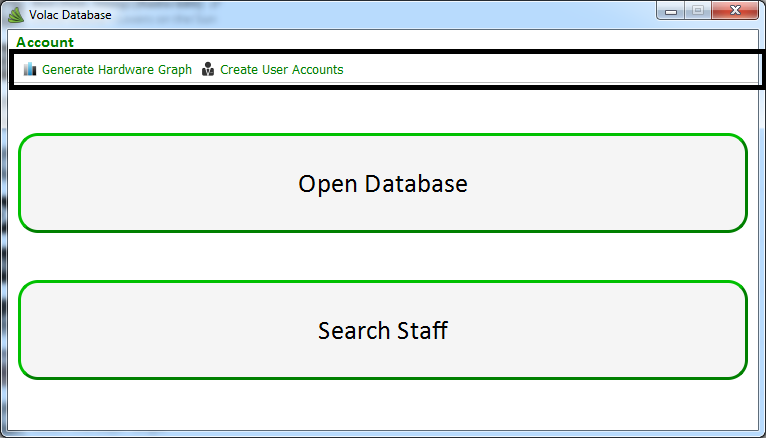
\includegraphics[width=\textwidth]{./Manual/Images/graph1.png}
\end{figure}

2) Press the "Generate Hardware Graph"

3) The graph should open, you may also save the image as .png

\begin{figure}[H]
    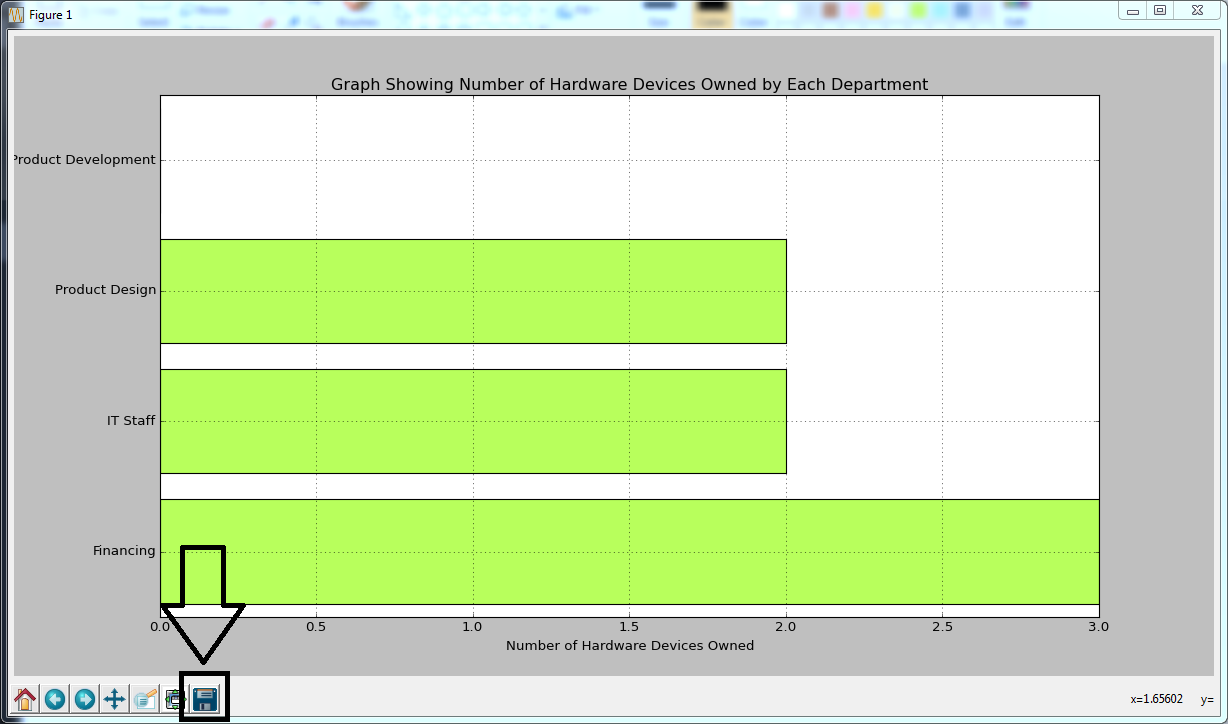
\includegraphics[width=\textwidth]{./Manual/Images/graph2.png}
\end{figure}

4) Close the graph by pressing the "X" button on the window

\subsubsection{How do I add new accounts to the system?}\label{accountcreate}

1) From anywhere in the Admin interface locate the toolbar

\begin{figure}[H]
    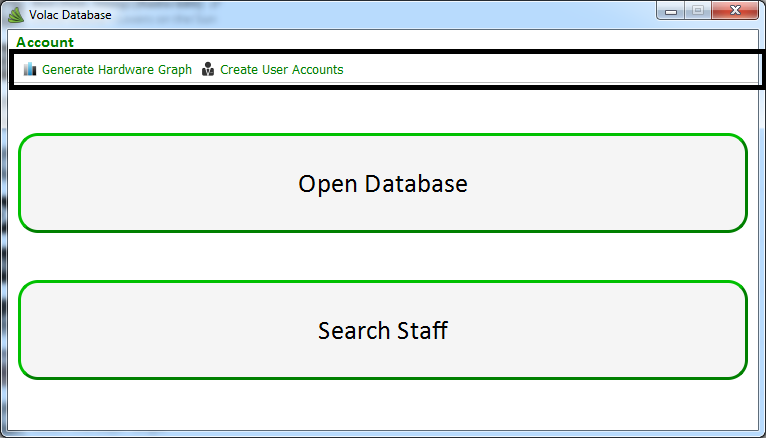
\includegraphics[width=\textwidth]{./Manual/Images/graph1.png}
\end{figure}

2) Press the "Create User Accounts"

3) To add an account, the staff member must first be added to the staff table (see \ref{adddata})

4) Using the drop down box, fill in the staff details. The "Access Level" will provide access to different parts of the system so make sure it is correct! 

\begin{figure}[H]
    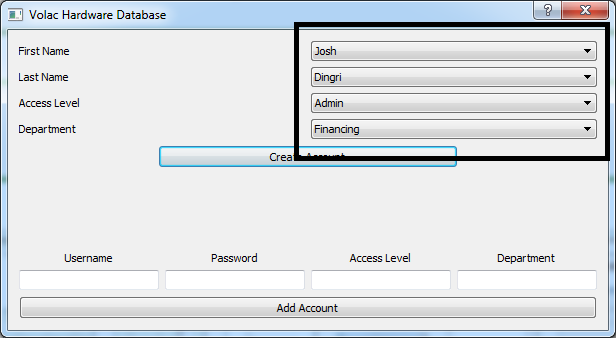
\includegraphics[width=\textwidth]{./Manual/Images/account2.png}
\end{figure}

5) Press "Create Account". This will generate login details

\begin{figure}[H]
    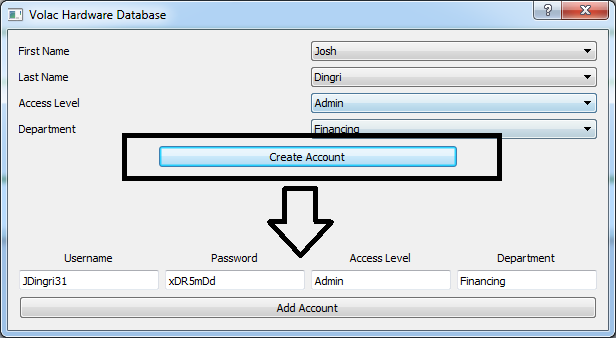
\includegraphics[width=\textwidth]{./Manual/Images/account3.png}
\end{figure}

6) You may change the details, however it is recommended that the password is kept the same since it is secure and randomly generated

7) Press "Add Account" to add the user to the system

\begin{figure}[H]
    \includegraphics[width=\textwidth]{./Manual/Images/account4.png}
\end{figure}

8) The user can now login with their details, make sure to tell the user to change their password when they first access the system

\subsubsection{What are primary and foreign keys and how do I use them?}\label{keys}

For the most part you will not have to worry about using primary and foreign keys. However when editing and deleting data it may be important to understand their use. Foreign keys will be presented when editing or deleting data, you will notice that under the "ID" fields there are numbers.

\begin{figure}[H]
    \includegraphics[width=\textwidth]{./Manual/Images/foreign.png}
\end{figure}

These numbers reference primary keys of other tables (which are basically unique identifiers for a record in that table). Therefore if you would like to edit a foreign key (to reference a different record) you will need to change the number to the primary key of your choice.

\begin{figure}[H]
    \includegraphics[width=\textwidth]{./Manual/Images/foreign2.png}
\end{figure}

You may not delete a record if it is referenced by a foreign key somewhere else.

\paragraph{Manager and Staff Interface Tutorial}

\subsubsection{I forgot my password, how do I recover it?}\label{recoveraccount}

1) On the login screen press the "Forgot username/password" button

\begin{figure}[H]
    \includegraphics[width=\textwidth]{./Manual/Images/forgot.png}
\end{figure}

2) Fill out all the details, make sure the email address is correct so that IT Staff can reply to your email, then click "Submit" (Press "Cancel" to close window)

\begin{figure}[H]
    \includegraphics[width=\textwidth]{./Manual/Images/forgot2.png}
\end{figure}

3) Await a response, the IT Staff will email you back with new account details over the next few days. If they do not reply within a week, email them directly.

\subsubsection{How do I view staff in my department?}\label{department}

This tutorial will only apply for managers.

1) Login to the manager interface

2) Click the "Department Information" button

\begin{figure}[H]
    \includegraphics[width=\textwidth]{./Manual/Images/department.png}
\end{figure}

3) From here you can view all staff in your department

\begin{figure}[H]
    \includegraphics[width=\textwidth]{./Manual/Images/department1.png}
\end{figure}

\subsubsection{How do I quick search for data when viewing Department Information?}\label{departquicksearch}

1) Enter the "Department Information" interface (see \ref{department})

2) To search for a field, enter text into the search box 

3) The table will automatically filter to show the text input

\begin{figure}[H]
    \includegraphics[width=\textwidth]{./Manual/Images/quicksearchdept.png}
\end{figure}

4) To show the whole table again, remove the text in the search box

\subsubsection{How do I view my own information?}\label{owninfo}

Both Managers and Staff can do this.

Managers:

1) Login to the manager interface

2) Click the "My Information" button 

\begin{figure}[H]
    \includegraphics[width=\textwidth]{./Manual/Images/myinfo.png}
\end{figure}

3) From here you can view your own devices stored in the database

\begin{figure}[H]
    \includegraphics[width=\textwidth]{./Manual/Images/myinfo2.png}
\end{figure}

Staff:

1) Login to the staff interface

2) The initial screen will be your own information

\begin{figure}[H]
    \includegraphics[width=\textwidth]{./Manual/Images/myinfostaff.png}
\end{figure}

3) From here you can view your own devices stored in the database

The quick search function is present on both layouts and you can use the search box to filter information. Simply enter text in the search box to filter the table.

\subsubsection{How do I report a bug?}\label{bugreport}

1) Press the "Help" menu on the menubar

\begin{figure}[H]
    \includegraphics[width=\textwidth]{./Manual/Images/bugreport.png}
\end{figure}

2) Select "Report Bug"


\begin{figure}[H]
    \includegraphics[width=\textwidth]{./Manual/Images/bugreport2.png}
\end{figure}


3) Fill out all fields and press "Send"


\begin{figure}[H]
    \includegraphics[width=\textwidth]{./Manual/Images/bugreport3.png}
\end{figure}


4) The IT Staff will look into the problem and resolve it as soon as possible

\subsubsection{How do I report incorrect information?}\label{incorrectinfo}

1) Press the "Help" menu on the menubar

\begin{figure}[H]
    \includegraphics[width=\textwidth]{./Manual/Images/bugreport.png}
\end{figure}

2) Select "Report Incorrect Information"

\begin{figure}[H]
    \includegraphics[width=\textwidth]{./Manual/Images/errorreport.png}
\end{figure}

3) Fill out all fields and press "Submit"

\begin{figure}[H]
    \includegraphics[width=\textwidth]{./Manual/Images/errorreport2.png}
\end{figure}

4) The IT Staff will look into the problem and resolve it as soon as possible

\subsection{Saving}

Editing data is the only situation where you will be required to save changes to the database manually, this is because it is a way of confirming that you want your edits to be committed to the database. You may also save graphs as .png in case you would like to use them in the future. Other than this, all saving is done automatically by the system (such as adding data and deleting data). This means that if the system was to crash, all data will still be saved to the database (as long as the user was not in the middle of editing data).

\subsection{Limitations}

The main limitation is the fact that the system is not online which means other colleagues cannot use the database at the same time, the client may expect this to have been completed but it can be done when I have more time to research this further. The client also may have expected that automatic emails work in a better way then they do currently, the fact that the user has to restart the system every day for the automated email to send may cause an inconvenience and they will want this fixed. Validation when editing data does not work at this point in time but it was not expected by the client so it may not be a problem of high priority.

\section{Error Recovery}

Certain problems may occur when using the system that will not display an error message, below I have stated how to recover from these errors so you may carry on using the program effectively. 

%include as many subsections as necessary for each error
\subsection{Problems Adding Accounts}

If you try and create a new account and then can't login with this new account it may be because the system has recognized that the username already exists. The system will not show an error but will not add this account in the database therefore it will not work. \newline

To solve the error simply try generating a new account with a different username. This should solve the problem. (see \ref{accountcreate} to create an account)

\subsection{Problems Adding Data}

Adding data should be work well but one problem that may arise is with inputs with combo boxes (drop-down boxes). If the default value is not changed in combo boxes, the field data will not be acknowledged. Solving this can be done easily:
\newline
1) Simply click the drop-down arrow and select an option

\begin{figure}[H]
    \includegraphics[width=\textwidth]{./Manual/Images/dropdownfix.png}
\end{figure}

2) If it was the default option that you wanted to select, click this item while in the drop-down list

\begin{figure}[H]
    \includegraphics[width=\textwidth]{./Manual/Images/dropdownfix2.png}
\end{figure}


3) Data should now add effectively

\subsection{Problems Opening Database File}

When opening the wrong database file you should be presented with an error which will not let the file open and ask you to try again (as shown below):

\begin{figure}[H]
    \includegraphics[width=\textwidth]{./Manual/Images/incorrectfile.png}
\end{figure}

Occasionally some files will not open and will not make an error message appear. More specifically this will happen if a file has the word "Volac" in it. 

\begin{figure}[H]
    \includegraphics[width=\textwidth]{./Manual/Images/incorrectfile2.png}
\end{figure}

\begin{figure}[H]
    \includegraphics[width=\textwidth]{./Manual/Images/incorrectfile3.png}
\caption{No error message is shown but the database has not been opened}
\end{figure}

If the database has not opened and no error was shown it may be because the wrong file has been chosen, to fix this problem simply attempt to re-open the correct file by following these steps below:

1) Press "Open Database"

\begin{figure}[H]
    \includegraphics[width=\textwidth]{./Manual/Images/opendb3.png}
\end{figure}

2) The problem should arise only if the incorrect file is opened, make sure the correct file has been chosen.

\begin{figure}[H]
    \includegraphics[width=\textwidth]{./Manual/Images/opendb4.png}
\end{figure}

3) The database should be open, you can now select a table. If the problem is still present, repeat from step 1 and make sure you are opening the correct file.

\begin{figure}[H]
    \includegraphics[width=\textwidth]{./Manual/Images/tabl2.png}
\end{figure}



\section{System Recovery}

\subsection{Backing-up Data}\label{backup}

Backing up the system is fairly simple, but it is important to note the system has no inbuilt back up system, therefore you will have to do this manually using the following steps below:

1) Navigate to where the system folder is located

\begin{figure}[H]
    \includegraphics[width=\textwidth]{./Manual/Images/backup1.png}
\end{figure}

\begin{figure}[H]
    \includegraphics[width=\textwidth]{./Manual/Images/backup2.png}
\end{figure}


2) Make sure the program has been closed and any saving has been made

3) Right click the system folder and press "Copy" (alternatively you may click the system folder and press "CTRL+C" on the keyboard)

\begin{figure}[H]
    \includegraphics[width=\textwidth]{./Manual/Images/backup3.png}
\end{figure}

4) Choose a location to back up the system to, the best option would be to save the folder on a removable flash drive or external hard drive. This way if the computer breaks, there is still a backup of the system


5) Right click any blank space inside the back up location and press "Paste" (alternatively you may press "CTRL+V" on the keyboard)

\begin{figure}[H]
    \includegraphics[width=\textwidth]{./Manual/Images/backup4.png}
\end{figure}

\begin{figure}[H]
    \includegraphics[width=\textwidth]{./Manual/Images/backup5.png}
\end{figure}

6) The system is now backed up, please see the below section on how to restore the system (\ref{restore})

\subsection{Restoring Data}\label{restore}

1) Navigate to where the backed up system folder is located (see (\ref{backup} for the backup tutorial)

\begin{figure}[H]
    \includegraphics[width=\textwidth]{./Manual/Images/restore1.png}
\end{figure}

2) Right click the folder and press "Copy" (alternatively you may click the system folder and press "CTRL+C" on the keyboard)

\begin{figure}[H]
    \includegraphics[width=\textwidth]{./Manual/Images/restore2.png}
\end{figure}

3) Navigate to where the system folder is located

4) You may now do one of two things:
\newline
\textbf{Method 1:}

1) Delete the system folder

\begin{figure}[H]
    \includegraphics[width=\textwidth]{./Manual/Images/restore1delete.png}
\end{figure}

2) Right click any blank space and press "Paste" (alternatively you may press "CTRL+V" on the keyboard)

\begin{figure}[H]
    \includegraphics[width=\textwidth]{./Manual/Images/restore1delete2.png}
\end{figure}

3) The new system will now replace the old system

\textbf{Method 2: (Preferred Option)}

1) Right click any blank space and press "Paste" (alternatively you may press "CTRL+V" on the keyboard)

2) You will now be asked to merge folders and overwrite files, select "Copy and Replace" and "Do this for the next X conflicts"

\begin{figure}[H]
    \includegraphics[width=\textwidth]{./Manual/Images/restore3.png}
\end{figure}

\begin{figure}[H]
    \includegraphics[width=\textwidth]{./Manual/Images/restore4.png}
\end{figure}

3) The new system will now replace the old system. 

\stopcontents[chapters]